% Sinh boi runners/make_paper1_figures.py; caption doi chieu bang
% runners/audit_figures.py. File rieng cho tung hinh de \input DUNG CHO
% trong than bai -- float cua LaTeX chi troi VE SAU, khai bao het o cuoi
% tai lieu thi ca 9 hinh don xuong cuoi va tran vao danh muc tai lieu.

\begin{figure*}[t]
  \centering
  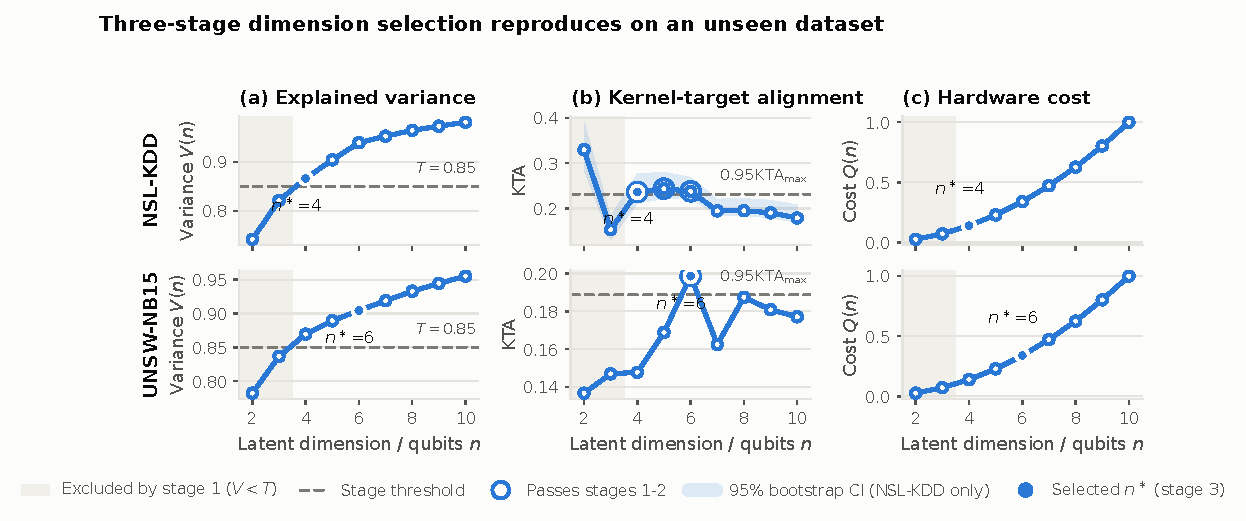
\includegraphics[width=\textwidth]{figs_revision/fig5_c1_dimension_selection.pdf}
  \caption{%
    \textbf{The three-stage dimension-selection rule, applied unchanged to two
    datasets.} Rows: NSL-KDD (top), UNSW-NB15 (bottom). Columns: (a) cumulative
    explained variance $V(n)$, (b) kernel--target alignment, (c) CNOT-weighted
    cost $Q(n)$. Stage~1 discards $V(n)<0.85$ (shaded), stage~2 keeps
    $\mathrm{KTA}\ge0.95\,\mathrm{KTA}_{\max}$ (open circles), stage~3 takes the
    cheapest survivor (filled). The same rule returns $n^{\ast}=4$ and
    $n^{\ast}=6$.}
  \label{fig:c1-selection}
\end{figure*}
